\documentclass[envcountsame,envcountsect]{llncs}
\usepackage{amssymb}
\usepackage{amsmath}
\usepackage{tikz}
\usetikzlibrary{topaths,calc}
\usepackage{pgfplots}
\pgfplotsset{compat=1.17}

\begin{document}

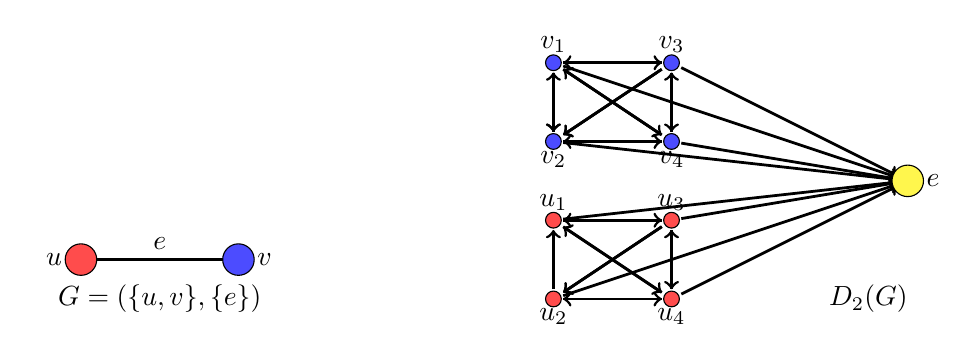
\begin{tikzpicture}
	\tikzstyle{edge} = [->, line width=1pt]
	\tikzstyle{uedge} = [-, line width=1pt]
	\node (v3) at (0,2) {};
	\node (e) at (10.5,3) {};
	\node (v5) at (6,4.5) {};
	\node (v6) at (6,3.5) {};
	\node (v7) at (7.5,4.5) {};

	\node (v8) at (7.5,3.5) {};


	\node (u5) at (6,2.5) {};
	\node (u6) at (6,1.5) {};
	\node (u7) at (7.5,2.5) {};

	\node (u8) at (7.5,1.5) {};

	\node (v4) at (2,2) {};

	\draw[edge] (v5) to (v6);
	\draw[edge] (v6) to (v5);
	\draw[edge] (v5) to (v7);
	\draw[edge] (v7) to (v5);
	\draw[edge] (v5) to (v8);
	\draw[edge] (v8) to (v5);
	\draw[edge] (v7) to (v6);
	\draw[edge] (v7) to (v6);
	\draw[edge] (v8) to (v6);
	\draw[edge] (v6) to (v8);
	\draw[edge] (v7) to (v8);
	\draw[edge] (v8) to (v7);


	\draw[edge] (v5) to (v6);
	\draw[edge] (u6) to (u5);
	\draw[edge] (u5) to (u7);
	\draw[edge] (u7) to (u5);
	\draw[edge] (u5) to (u8);
	\draw[edge] (u8) to (u5);
	\draw[edge] (u7) to (u6);
	\draw[edge] (u7) to (u6);
	\draw[edge] (u8) to (u6);
	\draw[edge] (u6) to (u8);
	\draw[edge] (u7) to (u8);
	\draw[edge] (u8) to (u7);

	\draw[edge] (u5) to (e);
	\draw[edge] (u6) to (e);
	\draw[edge] (u7) to (e);
	\draw[edge] (u8) to (e);
	\draw[edge] (v5) to (e);
	\draw[edge] (v6) to (e);
	\draw[edge] (v7) to (e);
	\draw[edge] (v8) to (e);

	\draw[uedge] (v3) to (v4);




	\filldraw[fill=yellow!70] (e) circle (0.2) node [right] {$~e$};

	\foreach \v in {3,4,...,8} {
		\fill (v\v) circle (0.1);

	}

	\foreach \u in {5,6,...,8} {
		\fill (u\u) circle (0.1);
	}

	\filldraw[fill=red!70] (v3) circle (0.2) node [left] {$ ~u~ $};
	\filldraw[fill=blue!70] (v4) circle (0.2) node [right] {$ ~v$};

	\filldraw[fill=blue!70](v5) circle (0.1) node [above] {$v_1$};
	\filldraw[fill=blue!70] (v6) circle (0.1) node[below] {$v_2$};
	\filldraw[fill=blue!70] (v7) circle (0.1) node[above] {$v_3$};
	\filldraw[fill=blue!70] (v8) circle (0.1) node [below] {$v_4$};

	\filldraw[fill=red!70](u5) circle (0.1) node  [above] {$u_1$};
	\filldraw[fill=red!70] (u6) circle (0.1) node [below] {$u_2$};
	\filldraw[fill=red!70] (u7) circle (0.1) node  [above] {$u_3$};
	\filldraw[fill=red!70] (u8) circle (0.1) node [below] {$u_4$};




	%	
	\node at (1,2.2) {$e$};

	\node at (1,1.5) {$G = (\{u,v\}, \{e\})$};


	\node at (10,1.5) {$D_2(G)$};


\end{tikzpicture}

\end{document}